\section{Early Science Data Products}
\label{sec:data}

All Rubin Observatory LSST data products are produced by the LSST Science Pipelines, \cite{2019ASPC..523..521B,2018PASJ...70S...5B}.
For an introduction to the LSST data products, see \citet{RubinDataProductsAbridged} and for a detailed description, see the LSST \dpdd,  \citet{LSE-163}.
Here we provide a summary of the data products that are expected to be made available as part of the Early Science Program.

Each pre-operations data preview and survey data release will be accompanied by its own release-specific DPDD, giving e.g. the  database schema for the catalogs included in that dataset.
For an example data release DPDD, see the online DP0.2 documentation \footnote{\url{https://dp0-2.lsst.io/data-products-dp0-2/}}.

The Rubin data rights policy is described in  \cite{RDO-013}.

%\subsection{Prompt data products}
% TODO make sure Alerts are described and that they are decoupled from a DP/
%
%Data products for transients, variable, and moving objects will be primarily produced by the Prompt Processing pipelines, which will perform reduction, calibration, difference image analysis (DIA), source detection and measurement, and alert distribution within 60 seconds of image readout.
%They include \emph{images}, \emph{catalogs} and \emph{alerts}. 
%
%During routine LSST operations, prompt image data products will be made available 80 hours following camera readout.
%They include raw images, processed single visit images (PVIs), difference images, and template images.
%Access to unvetted PVIs and difference images in the first 6 months of the LSST is still to be decided.
%Prompt image products are proprietary with the exception of  alert postage stamps, which are distributed in the alert stream and recorded in the alert database.
%The image differencing source (\DIASource), forced photometry (\DIAForcedSource), and object (\DIAObject and \SSObject) catalog data products are all public and will be available after 24 hours.
%Rubin Data Rights holders can access both prompt image and catalog data products via the Rubin Science Platform (\S~\ref{ssec:dataaccess}) and query using VO interfaces.
%
%Alerts are triggered by sources detected in difference images with a SNR>5 and transmitted to Rubin community alert brokers \footnote{Alert brokers are software systems that will ingest, process, and serve astronomical alerts from Rubin Observatory and other surveys to the broader scientific community.}.
%Typical broker functionality includes cross-match association with archival catalogs, the identification and prioritization of objects in need of follow-up observations, and photometric classification based on light-curve analysis.`
%Seven community alert brokers will receive direct access to the full stream and a further two will operate downstream of a full-stream broker. 
%For a full list of Rubin community brokers, see \url{https://www.lsst.org/scientists/alert-brokers}
%
%Alert packets transmitted to these brokers are world-public.
%Similarly, daily Solar System Processing identifies new Solar System Objects from difference image sources and reports those publicly to the Minor Planet Center.
%
%Alert production will begin shortly after System First Light, initially at low latency and limited volume but with both ramping up continuously through commissioning and into the first year of the survey.
%In this way, Alert production and distribution is decoupled from the Data Preview schedule.
%
% %In the tables below, we indicate what kind of Alert stream can be expected during each data preview ``era,'' defined as the time period within which that data preview's images are obtained.
%Note that the DP1 era is {\it very short}: the data products released in DP1 will be generated from relatively few observations taken in the few days around System First Light.
%
% Replace with a discussion of a bespoke PP to run for DP1 to optimize usefulness of the data products
%
%As such, it may not make much sense to run the Prompt Processing pipeline on the DP1 images.
%Instead, the DP1 data products will be generated with an abbreviated Data Release Processing pipeline, and focus on processed visit images and associated Source catalogs intended to support initial low-level investigations of Rubin's observational and instrumental effects.
%Then, the DP2 observations (commissioning's ``system optimization'' and Science Validation surveys) will be able to support prompt processing and alert generation shortly after System First Light, as well as investigation of the properties of the coadded images generated and Difference Image Analysis performed.
% % DRP image differencing on the First Light image time series would enable some limited initial time domain science with DP1, but is not planned at this time. 

\subsection{Data Release data products}

Static science datasets for Early Science will flow from science-grade data taken during the System Optimization' and Science Validation surveys during commissioning.
Images and catalogs from the DRP of the commissioning data will be made available to data rights holders in the form of Data Previews via the access mechanisms described in \S~\ref{ssec:dataaccess}.
Due to the relatively short time periods available for commissioning observations (\S~\ref{ssec:scenarios}), these Data Previews will necessarily be limited in their area and temporal coverage relative to full Data Releases, however all Data Preview data products will be in the same science data model format as for future Data Releases.

\subsection{Summary of expected Early Science Data Products} \label{ssec:dataproductsummary}
The tables in this section outline which data products can be expected in each Data Preview and Data Release, and on what time scale.
Following the replan of the construction project and the descoping of ComCam on-sky observations, the exact Data products to be released with Data Preview 1 are still under discussion.

\begin{table}
\caption{Summary of data products expected in each data preview and early survey data release, as of January 2023.
In the case of DP1, these expectations come with considerable uncertainty: see Table~\ref{tab:dp-one-products} for more on this.}
\label{tab:summary}
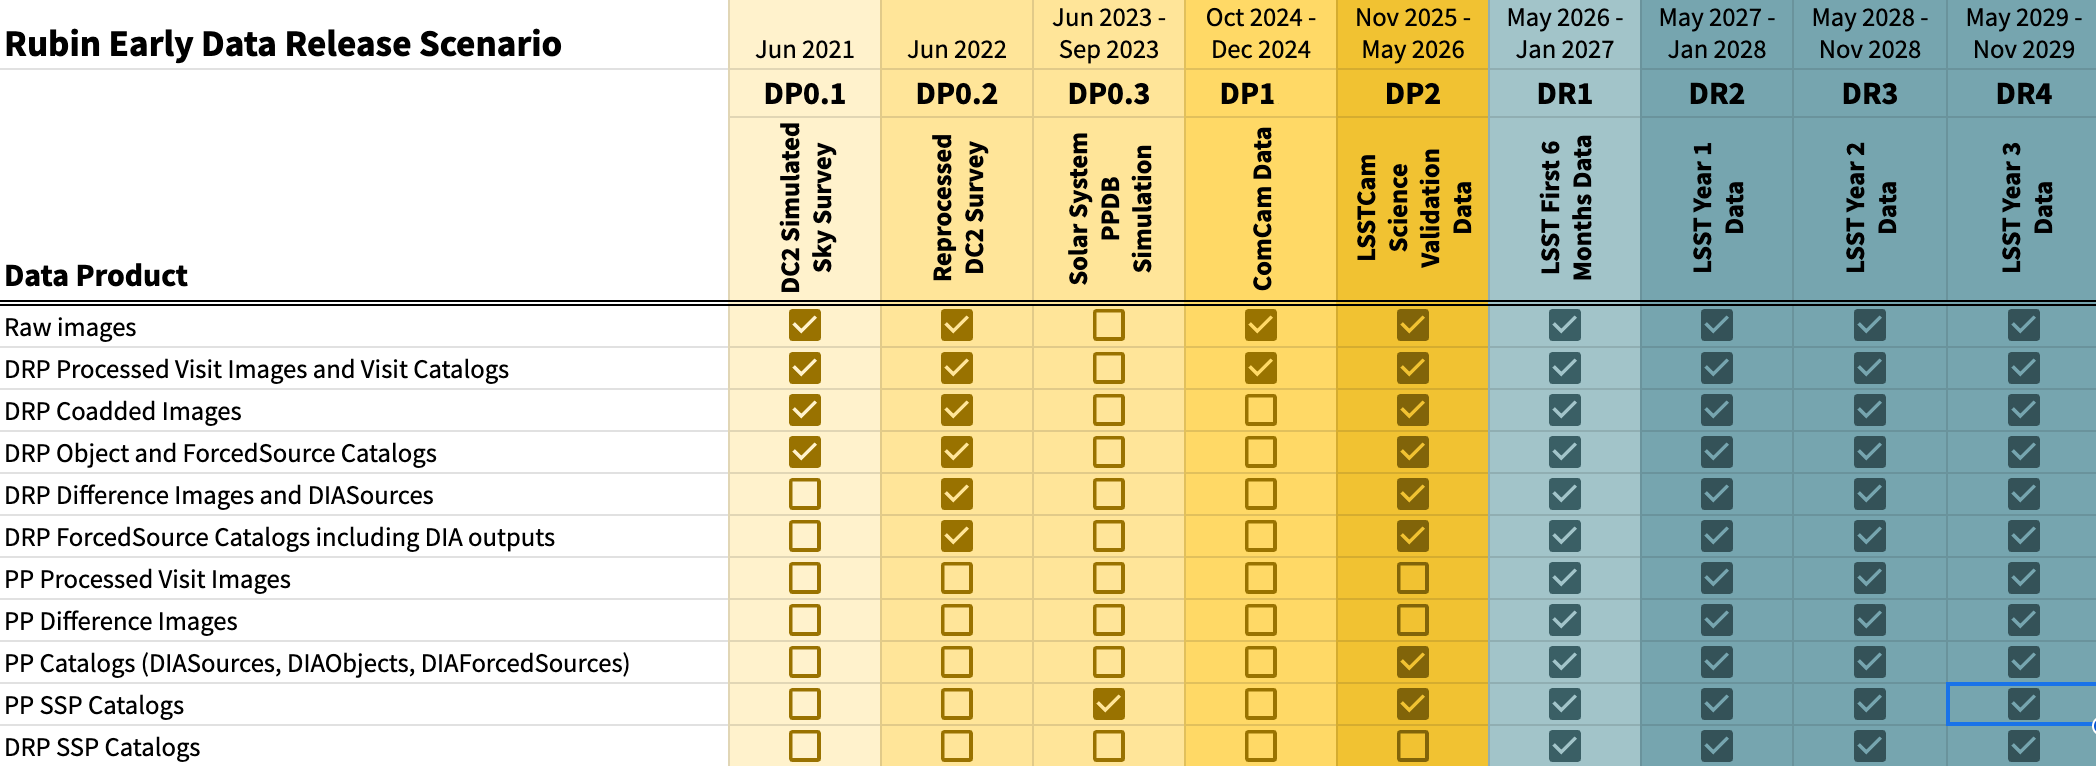
\includegraphics[width=\linewidth]{figures/DPR-summary}
\end{table}

\begin{table}
\caption{Summary of data products expected in DP0.3, as of January 2023.
DP0.3 will be planned in detail during 2023.}
\label{tab:dp-zpthree-products}
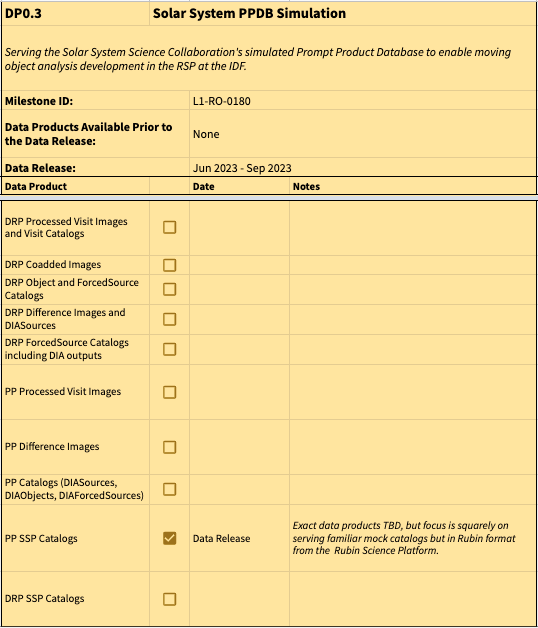
\includegraphics[width=\linewidth]{figures/DP0_3-products}
\end{table}

\begin{table}
\caption{Summary of data products expected in DP1, as of January 2023.
Note the high degree of uncertainty in this table: DP1 will be planned in detail during 2023. Shown here is the minimal set of data products that can be expected.}
\label{tab:dp-one-products}
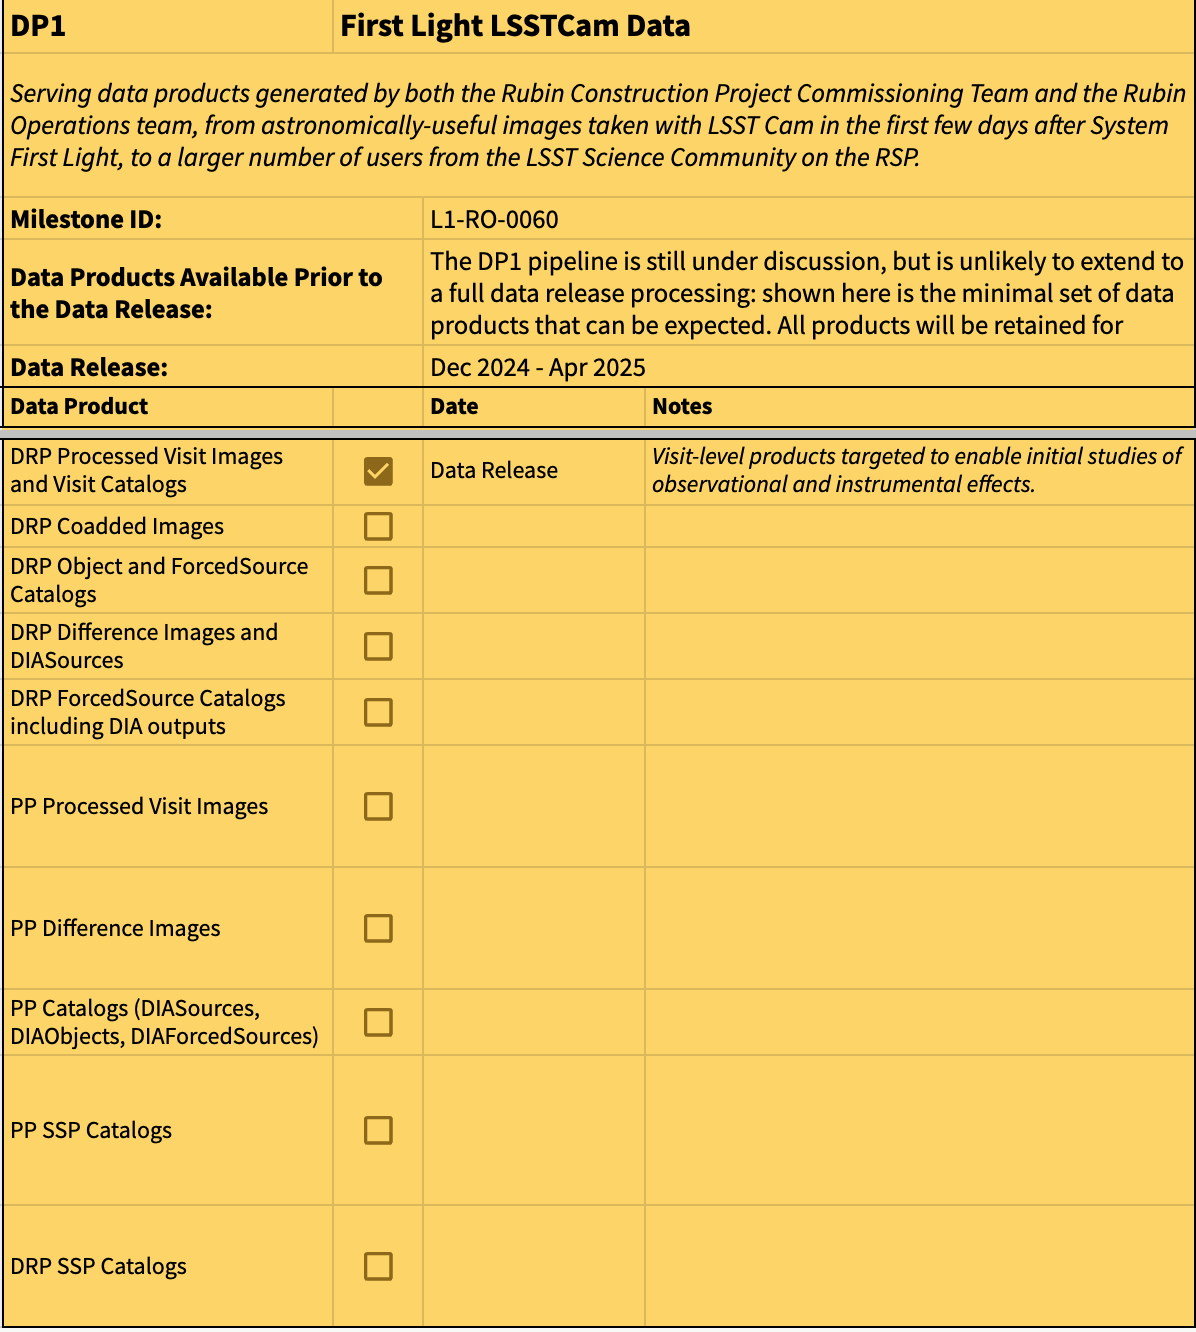
\includegraphics[width=\linewidth]{figures/DP1-products}
\end{table}

\begin{table}
\caption{Summary of data products expected in DP2, as of January 2023.}
\label{tab:dp-two-products}
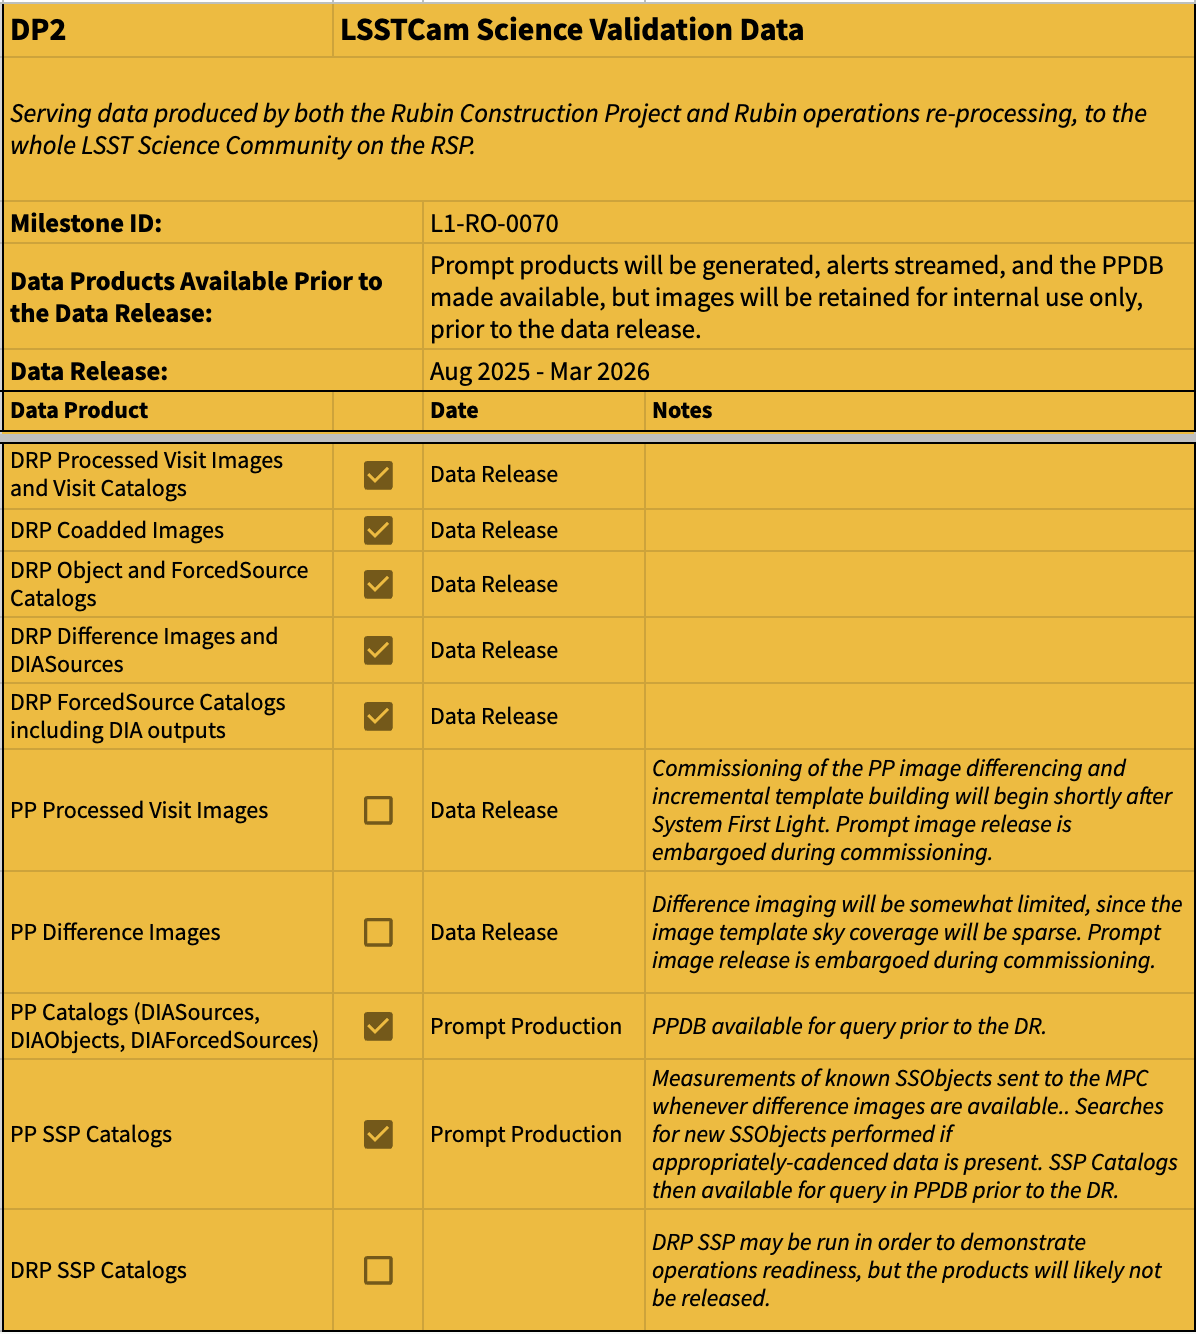
\includegraphics[width=\linewidth]{figures/DP2-products}
\end{table}

\begin{table}
\caption{Summary of data products expected in DR1, as of January 2023.}
\label{tab:dr-one-products}
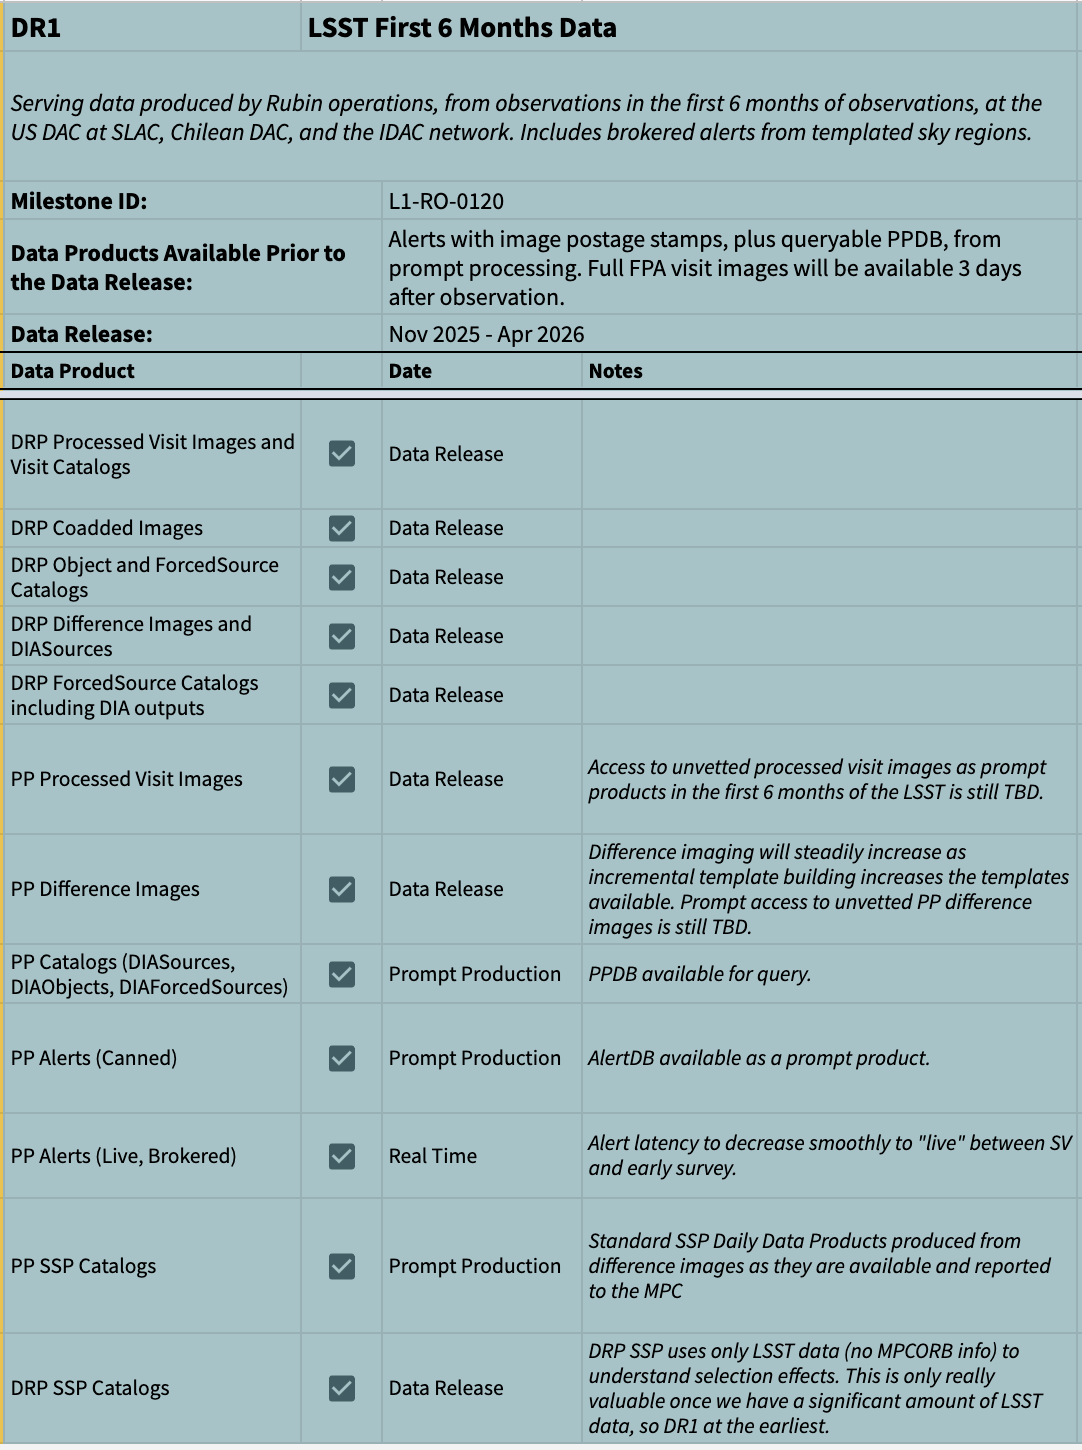
\includegraphics[width=\linewidth]{figures/DR1-products}
\end{table}


\subsection{Access to Early Science  Data Products} \label{ssec:dataaccess}
Alerts are fully world-public and will be accessible via one or more of the nine Rubin-endorsed Community Brokers\footnote{See \url{https://www.lsst.org/scientists/alert-brokers}}.
All other data products listed in \S~\ref{ssec:dataproductsummary} will be accessible to Rubin Data Rights community via the Rubin Science Platform (RSP), \citep{LSE-319}.

DP0.1 and DP0.2 are available via the RSP running at the US Data Access Center (US DAC), hosted on the Google Cloud Platform.
During pre-operations, Rubin is also using Google Cloud resources for some image processing runs (including DP0.2), as its ``Interim Data Facility'' (IDF).
Data processing is now in transition to the US Data Facility at SLAC, and the DP1 and DP2 processing will be carried out there.
(The France Data Facility at CC-IN2P3 in Lyon, and the UK Data Facility on the IRIS network, are also being commissioned in parallel in time to participate in survey data processing.)
Rubin data will continue to be served from the US DAC throughout pre-operations and into the LSST survey.
An assortment of Rubin Independent Data Access Centers (IDACs) is also under construction, to provide additional user computing resources to LSST users around the globe.
